\subsection{4.4-1}
    The recursion tree looks like: \\
    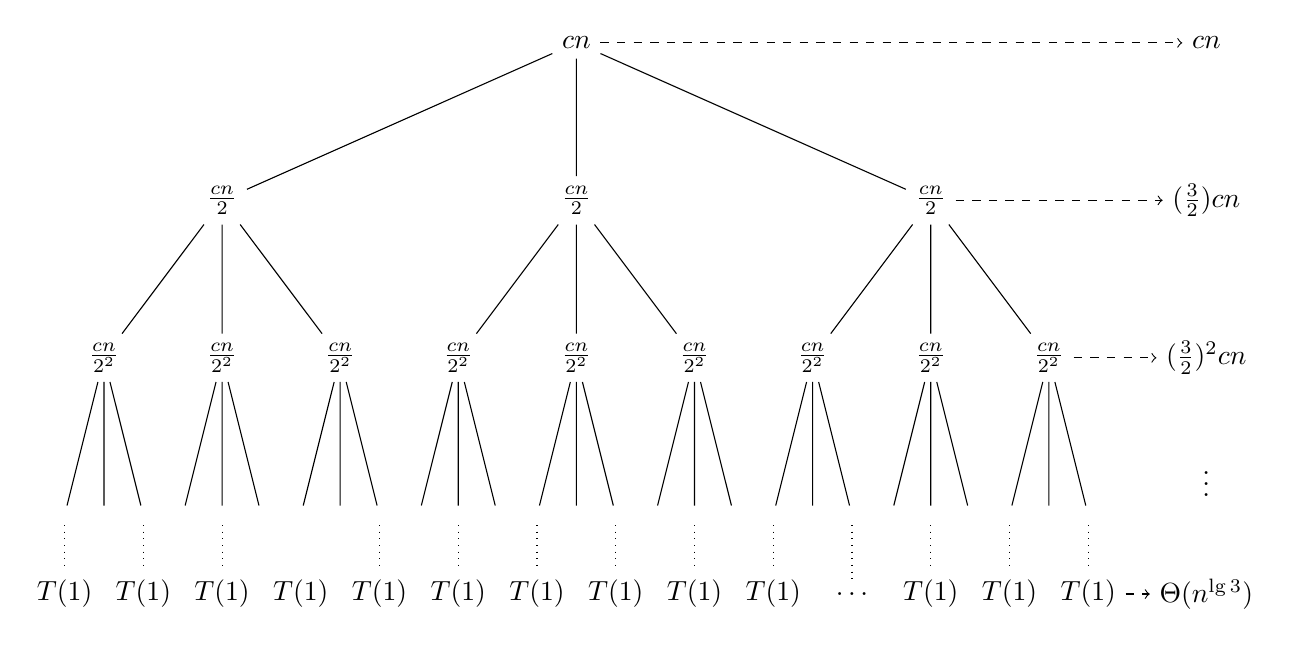
\begin{tikzpicture}[
        level 1/.style={sibling distance=4.5cm, level distance=2cm},
        level 2/.style={sibling distance=1.5cm, level distance=2cm},
        level 3/.style={sibling distance=0.5cm, level distance=2cm},
        level 4/.style={sibling distance=0.5cm, level distance=0cm},
        level 5/.style={sibling distance=0.5cm, level distance=1cm},
        level 19/.style={sibling distance=0.5cm, level distance=1.5cm},
        level 22/.style={sibling distance=0.5cm, level distance=2cm},
    ]
    \node (a) {$cn$}
        child {node {$\frac{cn}{2}$}
            child {node {$\frac{cn}{2^2}$}
                child {node {}
                    child [grow=down] {node {} edge from parent[draw=none]
                        child [grow=down]{node {$T(1)$} edge from parent[dotted]}
                    child [grow=right] {node {} edge from parent[draw=none]
                        child [grow=down]{node {$T(1)$} edge from parent[dotted]}
                    child [grow=right] {node {} edge from parent[draw=none]
                        child [grow=down]{node {$T(1)$} edge from parent[dotted]}
                    child [grow=right] {node {} edge from parent[draw=none]
                        child [grow=down]{node {$T(1)$} edge from parent[draw=none]}
                    child [grow=right] {node {} edge from parent[draw=none]
                        child [grow=down]{node {$T(1)$} edge from parent[dotted]}
                    child [grow=right] {node {} edge from parent[draw=none]
                        child [grow=down]{node {$T(1)$} edge from parent[dotted]}
                    child [grow=right] {node {} edge from parent[draw=none]
                        child [grow=down]{node {$T(1)$} edge from parent[dotted]}
                    child [grow=right] {node {} edge from parent[draw=none]
                        child [grow=down]{node {$T(1)$} edge from parent[dotted]}
                    child [grow=right] {node {} edge from parent[draw=none]
                        child [grow=down]{node {$T(1)$} edge from parent[dotted]}
                    child [grow=right] {node {} edge from parent[draw=none]
                        child [grow=down]{node {$T(1)$} edge from parent[dotted]}
                    child [grow=right] {node {} edge from parent[draw=none]
                        child [grow=down]{node {$\dots$} edge from parent[dotted]}
                    child [grow=right] {node {} edge from parent[draw=none]
                        child [grow=down]{node {$T(1)$} edge from parent[dotted]}
                    child [grow=right] {node {} edge from parent[draw=none]
                        child [grow=down]{node {$T(1)$} edge from parent[dotted]}
                    child [grow=right] {node {} edge from parent[draw=none]
                        child [grow=down]{node (g) {$T(1)$} edge from parent[dotted]
                            child [grow=right] {node (h) {$\Theta(n^{\lg 3})$} edge from parent[draw=none]
                                child [grow=up] {node {$\vdots$} edge from parent[draw=none]
                                child [grow=up] {node (f) {$(\frac{3}{2})^2cn$} edge from parent[draw=none]
                                child [grow=up] {node (d) {$(\frac{3}{2})cn$} edge from parent[draw=none]
                                child [grow=up] {node (b) {$cn$} edge from parent[draw=none]
                                } } } }
                            }
                        }
                    } } } } } } } } } } } } } }
                }
                child {node {}}
                child {node {}}
            }
            child {node {$\frac{cn}{2^2}$}
                child {node {}}
                child {node {}}
                child {node {}}
            }
            child {node {$\frac{cn}{2^2}$}
                child {node {}}
                child {node {}}
                child {node {}}
            }
        }
        child {node {$\frac{cn}{2}$}
            child {node {$\frac{cn}{2^2}$}
                child {node {}}
                child {node {}}
                child {node {}}
            }
            child {node {$\frac{cn}{2^2}$}
                child {node {}}
                child {node {}}
                child {node {}}
            }
            child {node {$\frac{cn}{2^2}$}
                child {node {}}
                child {node {}}
                child {node {}}
            }
        }
        child {node (c) {$\frac{cn}{2}$}
            child {node {$\frac{cn}{2^2}$}
                child {node {}}
                child {node {}}
                child {node {}}
            }
            child {node {$\frac{cn}{2^2}$}
                child {node {}}
                child {node {}}
                child {node {}}
            }
            child {node (e) {$\frac{cn}{2^2}$}
                child {node {}}
                child {node {}}
                child {node {}
                }
            }
        };
    \draw[dashed, ->] (a) -- (b);
    \draw[dashed, ->] (c) -- (d);
    \draw[dashed, ->] (e) -- (f);
    \draw[dashed, ->] (g) -- (h);
    \end{tikzpicture}
    which indicates that the solution of the recurence is $O(n^{\lg 3})$ (the
    proof is similar to the one in page 90). \\
    Assuming that the solution of $T(n) = 3T(\floor{(n/2)}) + n$ is
    $O(n^{\lg 3})$, so for some positive constant $c$ and $n \ge n_0$, we have:
    \begin{align*}
        T(n) & \le 3c(\frac{n}{2})^{\lg 3} + n \\
             & = 3c\frac{n^{\lg 3}}{2^{\lg 3}} + n \\
             & = cn^{\lg 3} + n \\
             & = O(n^{\lg 3})
    \end{align*}
